\documentclass[12pt]{article}

\usepackage{polski}			% Polish characters
\usepackage[utf8]{inputenc}	% Polish characters
\usepackage{indentfirst}	% Indentation in first paragraph
\usepackage{graphicx}
\usepackage{geometry}
\usepackage{hyperref}

	
\graphicspath{{images}} %Setting the graphicspath

\hypersetup{
	linkcolor=black,
	colorlinks=true,
	urlcolor=blue,
	}
\urlstyle{same}

\begin{document}


\begin{titlepage} % Titlepage don't count to page numbering
	
	\center % Centre everything on the page
	
	%----------------------------------------------------------------------------------------
	%	Title
	
	\rule[1.0cm]{\textwidth}{1.0mm}
	
	{\huge\bfseries Olympus Movie}\\[0.5cm]
	
	\rule[1.5cm]{\textwidth}{1.0mm}
	%----------------------------------------------------------------------------------------	
	
	%----------------------------------------------------------------------------------------
	%	Logo
	
	
\includegraphics[scale=0.5]{logo.png}\\[1cm]
	
	%----------------------------------------------------------------------------------------
	
	%----------------------------------------------------------------------------------------
	%	Author(s)
	
	\begin{minipage}{0.4\textwidth}
		\begin{flushright}
			\large
			\textit{Autorzy}\\
			Jakub Nowak - Kierownik
			
			Marcelina Ziętal
			
			Dawid Polaczek
		\end{flushright}
	\end{minipage}
	%----------------------------------------------------------------------------------------
	
	%----------------------------------------------------------------------------------------
	%	Date
	
	\vspace{\fill}
	2022
	
	%----------------------------------------------------------------------------------------
	
	
\end{titlepage}
\begin{flushleft}

\newgeometry{tmargin=2.5cm, bmargin=2.5cm, lmargin=3cm, rmargin=1.5cm}
	%----------------------------------------------------------------------------------------
	%	Table of contents
	
	\tableofcontents
	\pagebreak
	%----------------------------------------------------------------------------------------
	
	%----------------------------------------------------------------------------------------
	%	Chapters

	\section{Słownik}	%rozpisać skróty i ujednolicić dokumentację
		Olympus Movie - autorska nazwa serwisu internetowego.
		
		Administrator - specjalny użytkownik posiadający rozszerzony zakres dostępnych funkcji.
		
		Pozycja - ogólna nazwa odnosząca się jednocześnie do filmów i seriali.
		
		Użytkownik - osoba korzystająca z serwisu. W jego skład wchodzi użytkownik niezalogowany i użytkownik zalogowany. Każdy z nich posiada inne `funkcjonalności.
		
		Formularz -  służy do zbierania danych wprowadzanych przez użytkownika. Dane wejściowe użytkownika są najczęściej wysyłane do serwera w celu przetworzenia.
		
\pagebreak
	\section{Specyfikacja wymagań biznesowych}
	
		\subsection{Cel systemu}	%opis dlaczego taki system i jakie problemy rozwiazuje jego zbudowanie 
		Celem projektu "Olympus Movie" jest stworzenie strony internetowej poświęconej filmom, serialom oraz osobom uczestniczącym w ich tworzeniu. Użytkownik po zarejestrowaniu i zalogowaniu jest w stanie komentować, oceniać i recenzować pozycje.
	
	Każda osoba odwiedzająca stronę ma możliwość wyszukania pozycji na podstawie licznych filtrów. Podstawowe wyszukiwanie przeszukuje jedynie tytuły. Istniej możliwość wyszukiwania zaawansowanego w którym wyszukiwanie następuje po tagach lub gatunkach.
	
	Baza danych zawiera również informacje o aktorach, reżyserach, scenarzystach i innych osobach biorących udział w tworzeniu danej pozycji. Pozwala to na wyświetlenie pozycji w których grał konkretny aktor lub konkretna osoba brała udział w jego tworzeniu.
		
		\subsection{Wymagania funkcjonalne}
			\begin{itemize}
				\item Filtrowanie i sortowanie pozycji według wybranych kryteriów.
				\item Utworzenie/edycja/usunięcie konta użytkownika.
				\item Utworzenie/edycja/usunięcie pozycji.
				\item Utworzenie/edycja/usunięcie recenzji.
				\item Dodanie/edycja oceny danej pozycji.
				\item Komentowanie recenzji.
				\item Edycja/usunięcie dodanego komentarza.
				\item Tworzenie list pozycji.
			\end{itemize}
		
		\subsection{Wymagania niefunkcjonalne}
			\begin{itemize}
				\item Korzystanie z serwisu za pośrednictwem przeglądarki internetowej.
				\item Kompatybilność z przeglądarkami obsługującymi HTML 5.
				\item Przejrzysty interfejs użytkownika.
				\item Szybka reakcja na działania użytkownika.
				\item Stabilna dostępność do serwisu.
				\item Zapewnienie ciągłości dostępu do serwisu użytkownikom.
				\item Bezpieczeństwo danych logowania.
			\end{itemize}
		
		\subsection{Opis ograniczeń systemu}
			\begin{enumerate}
				\item Trailery oraz plakaty wyświetlane na stronie nie znajdują się w bazach danych. Przechowywane są jedynie linki do nich ze stron zewnętrznych.
				\item Brak listy znajomych lub obserwowanych użytkowników.
				\item Brak powiadomień.
				\item Brak ustawień. W tym zmiany języka.
				\item Brak zmiany motywu na stronie.
				\item Mocno ograniczony zakres bazy danych. Serwis nie posiada możliwości importowania pozycji z zewnętrznej strony. Wszystkie dane muszą zostać wprowadzone bezpośrednio w serwisie.					\item Do działania niezbędny jest dostęp do bazy danych.
				\item Ilość informacji składowanych w bazach danych szybko rośnie, co może powodować problemy w obsłudze.
			\end{enumerate}
					
		
\pagebreak
	\section{Dokumentacja techniczna}
		\subsection{Wybrane technologie}
		\begin{itemize}
			\item Docker -  środowisko do tworzenia aplikacji. Ułatwia pakowanie, tworzenie, dostarczanie i uruchamianie aplikacji ze wszystkimi jej zależnościami i wdrażanie jej jako pojedynczej jednostki. Posiada gotowe kontenery dla twórców aplikacji.
			\item ASP.NET Core - umożliwia tworzenie aplikacji internetowych i usług. Technologię można wdrażać w chmurze lub lokalnie. Całość zaprojektowana jest w sposób umożliwiający testowanie. Posiada wbudowane wstrzykiwanie zależności, niezbędne w przypadku tego projektu. Umożliwia hostowanie między inny Dockera.
			\item Microsoft SQL Server (MS SQL) = system do zarządzania bazą danych. Jest bardziej wydajny, niezawodny i skalowalny od większości tego typu systemów. Posiada prostą konfigurację. Usługa serwera jest podstawą platformy SQL Server. Realizowane są przez nią wszystkie zadania, które wiążą się z obsługą i utrzymaniem baz danych. Stanowi ona fundament, dlatego każde opiera się o trzon silnika bazy danych (Database Engine).
			\item React.js - javascriptowa biblioteka służąca do tworzenia interfejsów użytkownika. 
			\item Node.js - środowisko uruchomieniowe języka JavaScript po stronie serwera, które wykonuje kod JavaScript.
		\end{itemize}
		\subsection{Architektura systemu}
		Olympus Movie działa na podstawie mikroserwisów. Pozwalają one podzielić całość aplikacji na mniejsze, niezależne części. Ta architektura ułatwia testowanie ponieważ każdy z mikroserwisów można testować i wdrażać oddzielnie od pozostałych.
		
		Serwis używa Dockera dla mikroserwisów. Jest to jeden z najbardziej rozwijanych obecnie dostawców kontenerów co powoduje wsparcie społeczności na najwyższym poziomie. Potrzebuje mniej zasobów niż maszyny wirtualne co czyni go oszczędniejszym w użytkowaniu. Za jego pomocą można ułatwić ciągłą integrację i wdrażanie.

		Stosowanym wzorcem architektonicznym jest ECB(entity-control-boundary). Porządkuje klasy wchodzące w skład oprogramowania zgodnie z ich obowiązkami w realizacji przypadków użycia.
		\begin{itemize}
			\item Entity(encje) - obiekty reprezentujące dane systemowe, np.: User, Movie.
			\item Boundary(granice) - obiekt łączący się z aktorami systemowymi, między innymi: interfejs użytkownika, gateways(bramki sieciowe), serwerami proxy.
			\item Controlers(kontrolery) - obiekty pośredniczące między granicami i encjami. Aranżują wykonywanie poleceń pochodzących z granicy.
		\end{itemize}

		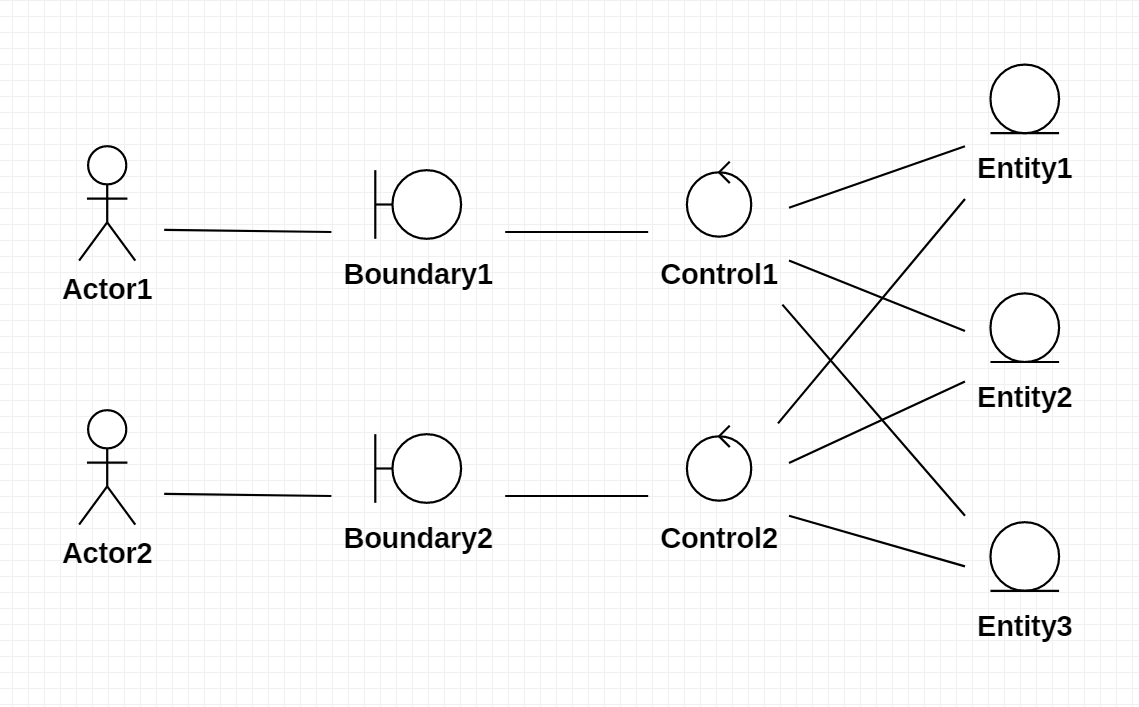
\includegraphics[scale=0.5]{ECB.png}

		\subsection{Diagramy przypadków użycia}
			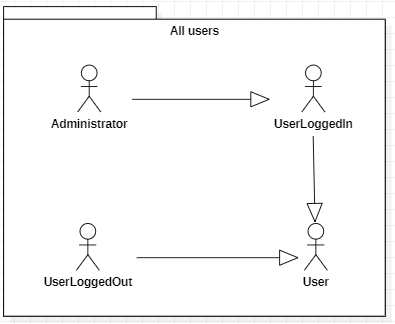
\includegraphics[scale=0.9]{UseCase_AllUsers.png} \linebreak
			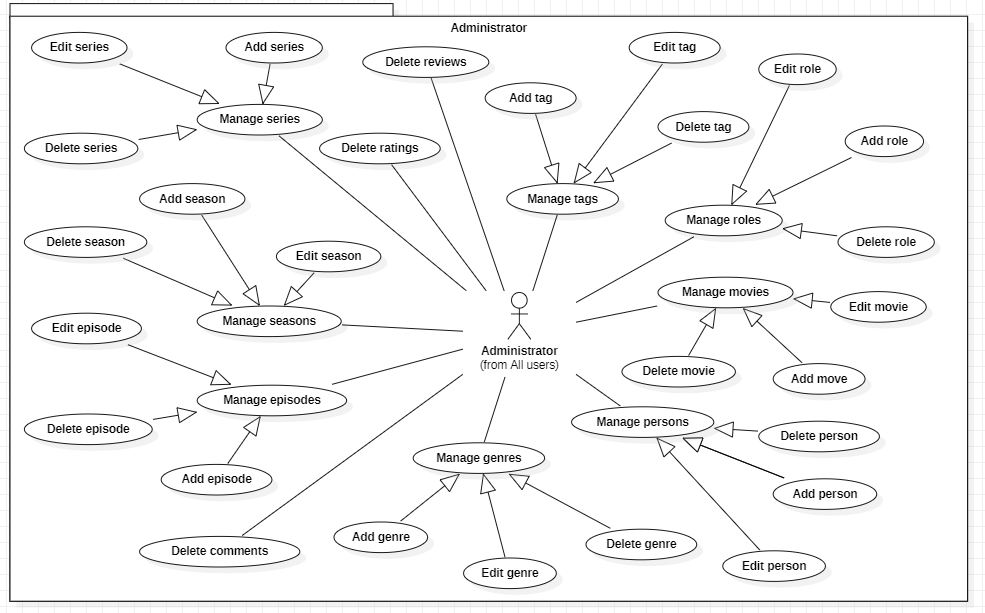
\includegraphics[scale=0.7]{UseCase_Administrator.png} \linebreak
			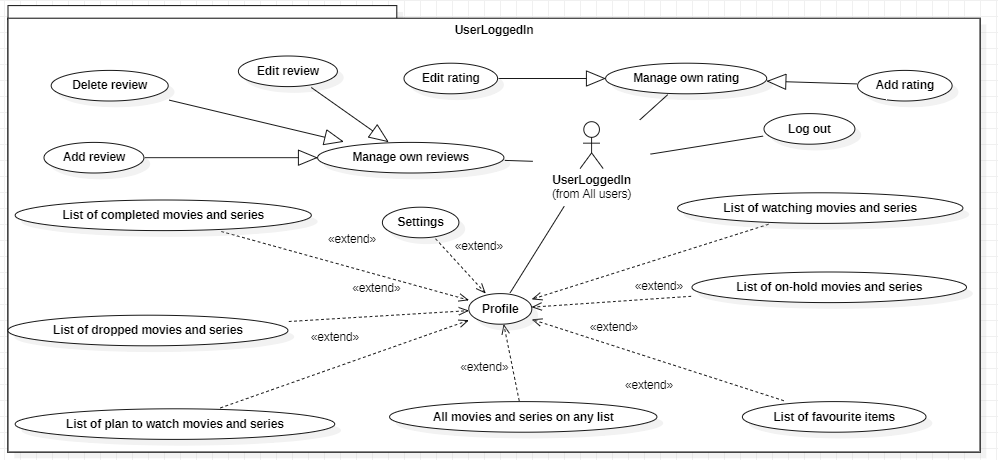
\includegraphics[scale=0.7]{UseCase_UserLoggedIn.png} \linebreak
			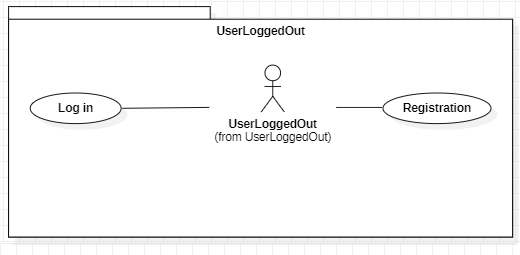
\includegraphics[scale=0.9]{UseCase_UserNotLoggedIn.png} \linebreak
			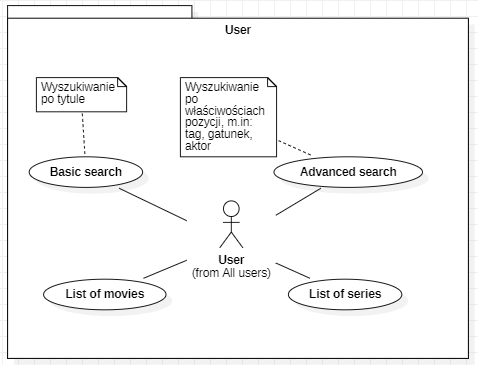
\includegraphics[scale=0.9]{UseCase_User.png} \linebreak
		
		\subsection{Diagram klas}
			\begin{center}
				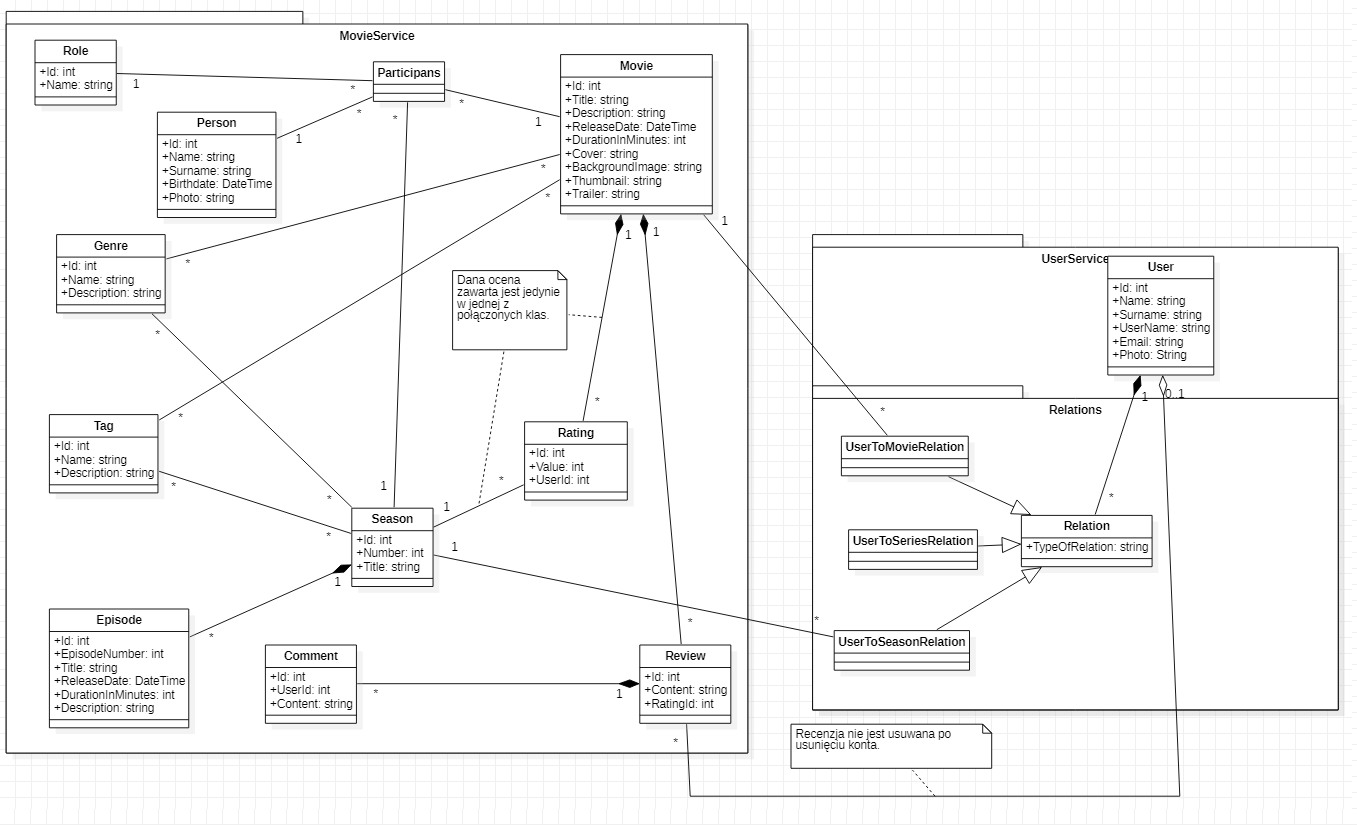
\includegraphics[scale=0.5]{Class_FilmsDataBase.png}
			\end{center}
		
		\subsection{Dokumentacja API}	%swaggers
		LINK DO SWAGGERA
\pagebreak
			
	\section{Dokumentacja użytkownika}
		\subsection{Funkcjonalność użytkownika anonimowego}
		\begin{itemize}
			\item Losowanie nazwy użytkownika podczas rejestracji.		
			Nazwa użytkownika losowana jest na podstawie wprowadzonego imienia i nazwiska. Pobierana jest losowa ilość znaków z imienia, następnie nazwiska. Do tak utworzonej nazwy dołączany jest numer z zakresu 1-1000. \linebreak`
			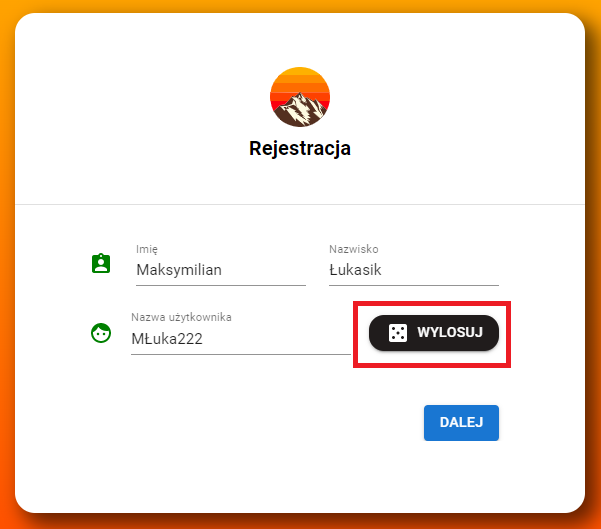
\includegraphics[scale=0.7]{WylosowanieNazwy.png} \linebreak
			\item Rejestracja.
			W prawym górnym roku strony kliknąć "REJESTRACJA". \linebreak
			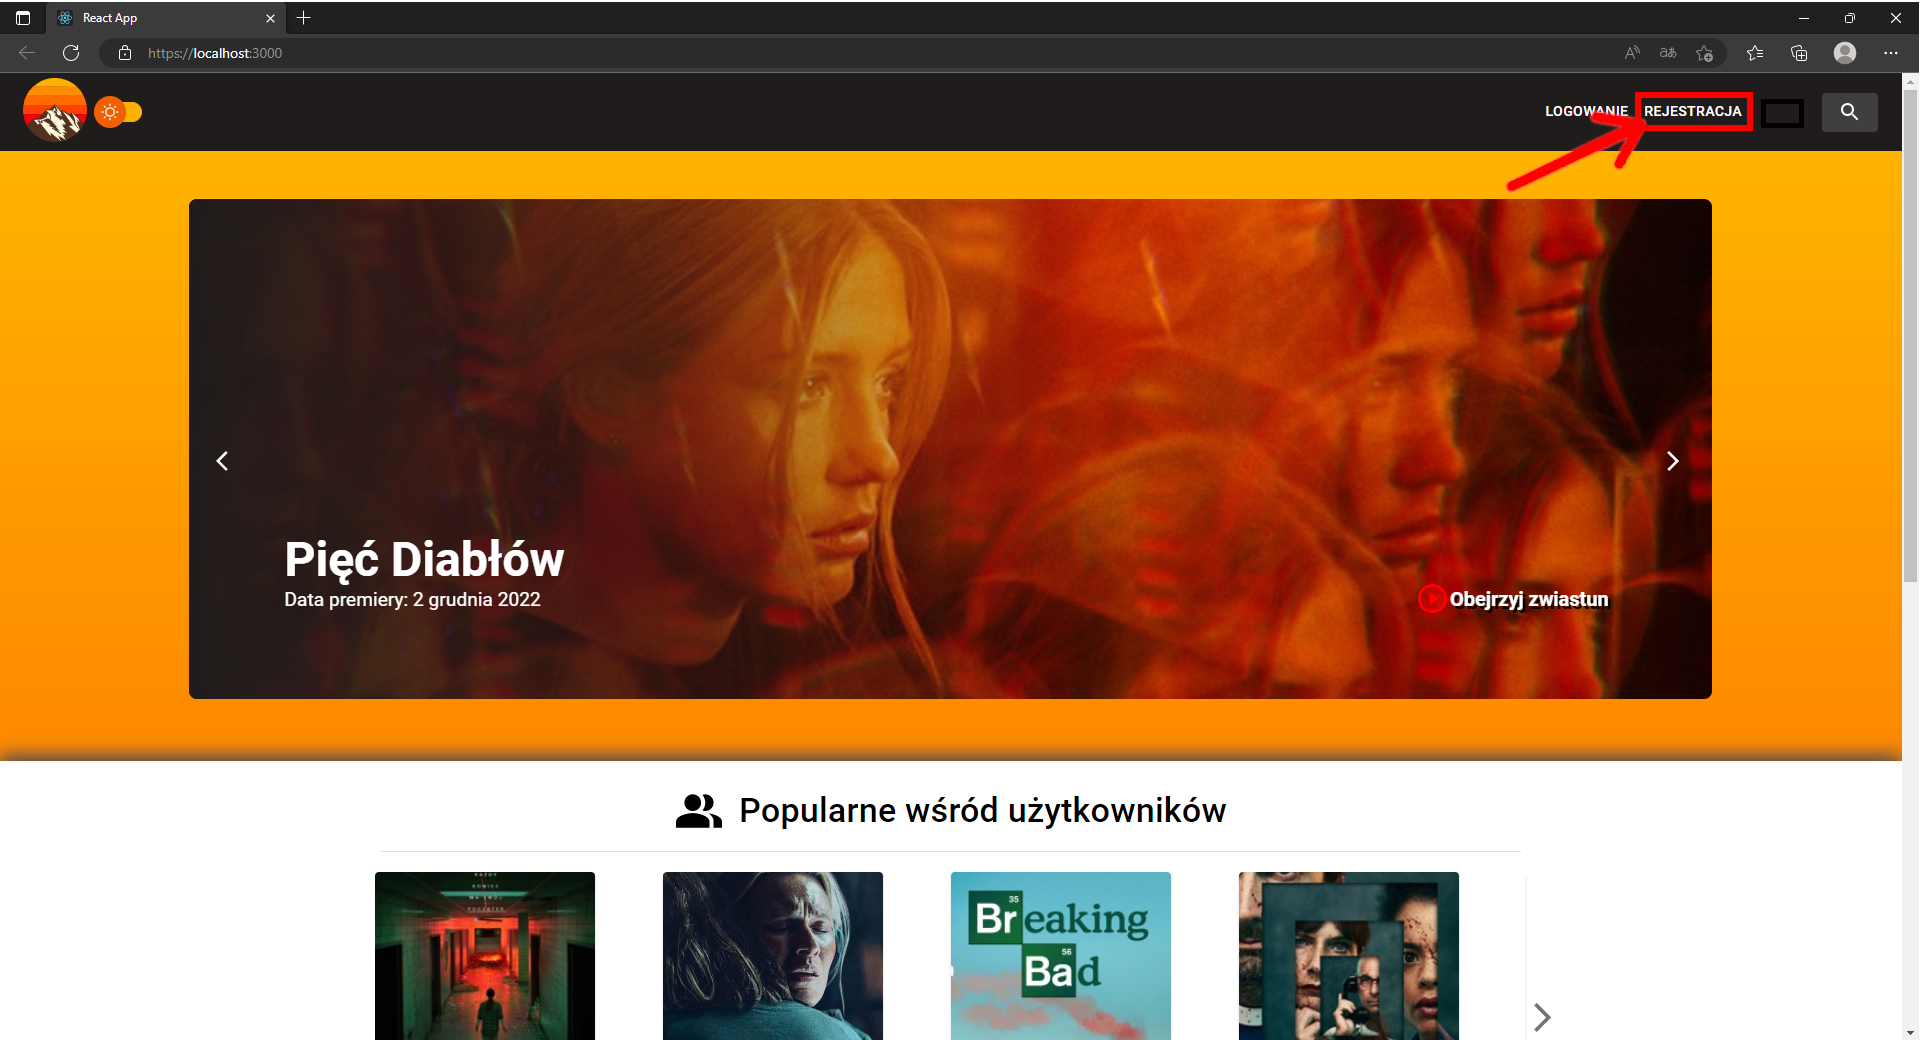
\includegraphics[scale=0.3]{Rejestracja1.png} \linebreak
			W pierwszej części formularza należy wypełnić wszystkie pola. Imię oraz nazwisko muszą posiadać co najmniej 2 znaki. Podana nazwa użytkownika powinna posiadać co najmniej 5 znaków i będzie niezbędna podczas logowania. Istnieje możliwość losowego wybrania nazwy użytkownika. \linebreak
			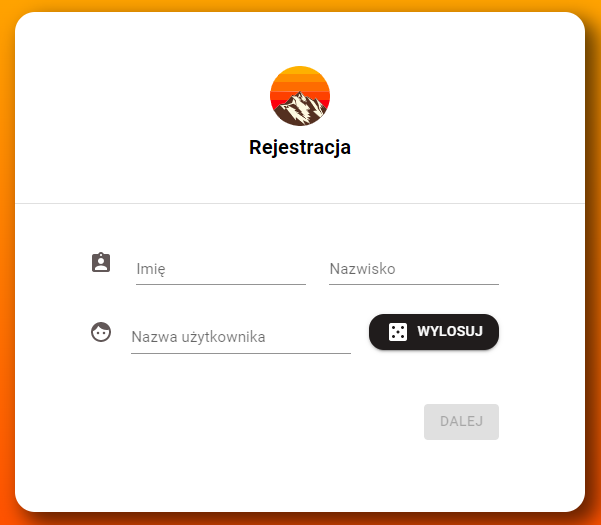
\includegraphics[scale=0.7]{Rejestracja2.png} \linebreak
			W drugiej części formularza należy wypełnić wszystkie pola. Adres e-mail oraz hasło należy wpisać dwukrotnie w celu uniknięcia literówki. Klikając na ikonę oka możemy włączyć podgląd hasła. Hasło powinno mieć co najmniej 6 znaków w tym co najmniej po jednej wielkiej i małej literze oraz jeden znak specjalny.\linebreak
			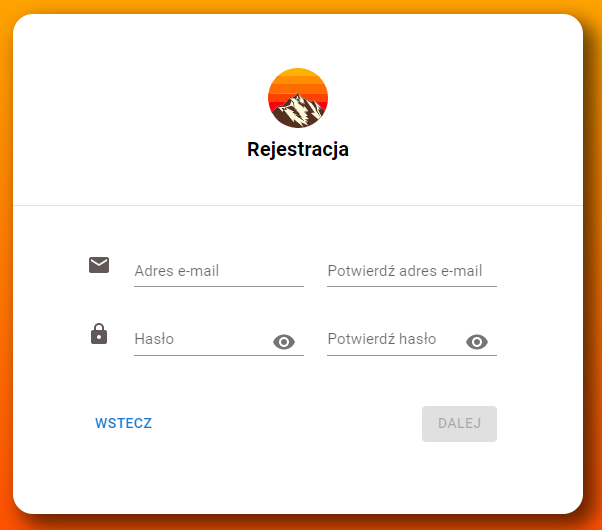
\includegraphics[scale=0.7]{Rejestracja3.png} \linebreak
			W ostatniej części formularza należy podać datę urodzenia. Po kliknięciu na "ZAKOŃCZ" rejestracja zostanie zakończona.\linebreak
			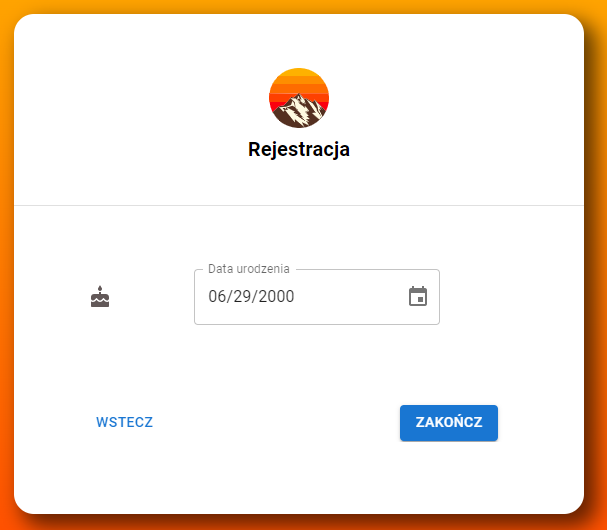
\includegraphics[scale=0.7]{Rejestracja4.png} \linebreak
			W przypadku źle przeprowadzonej rejestracji w lewym dolnym rogu zostanie wyświetlony komunikat. Jeśli rejestracja zakończy się sukcesem użytkownik zostanie przekierowany do strony głównej i będzie mógł się zalogować na swoje konto.\linebreak
			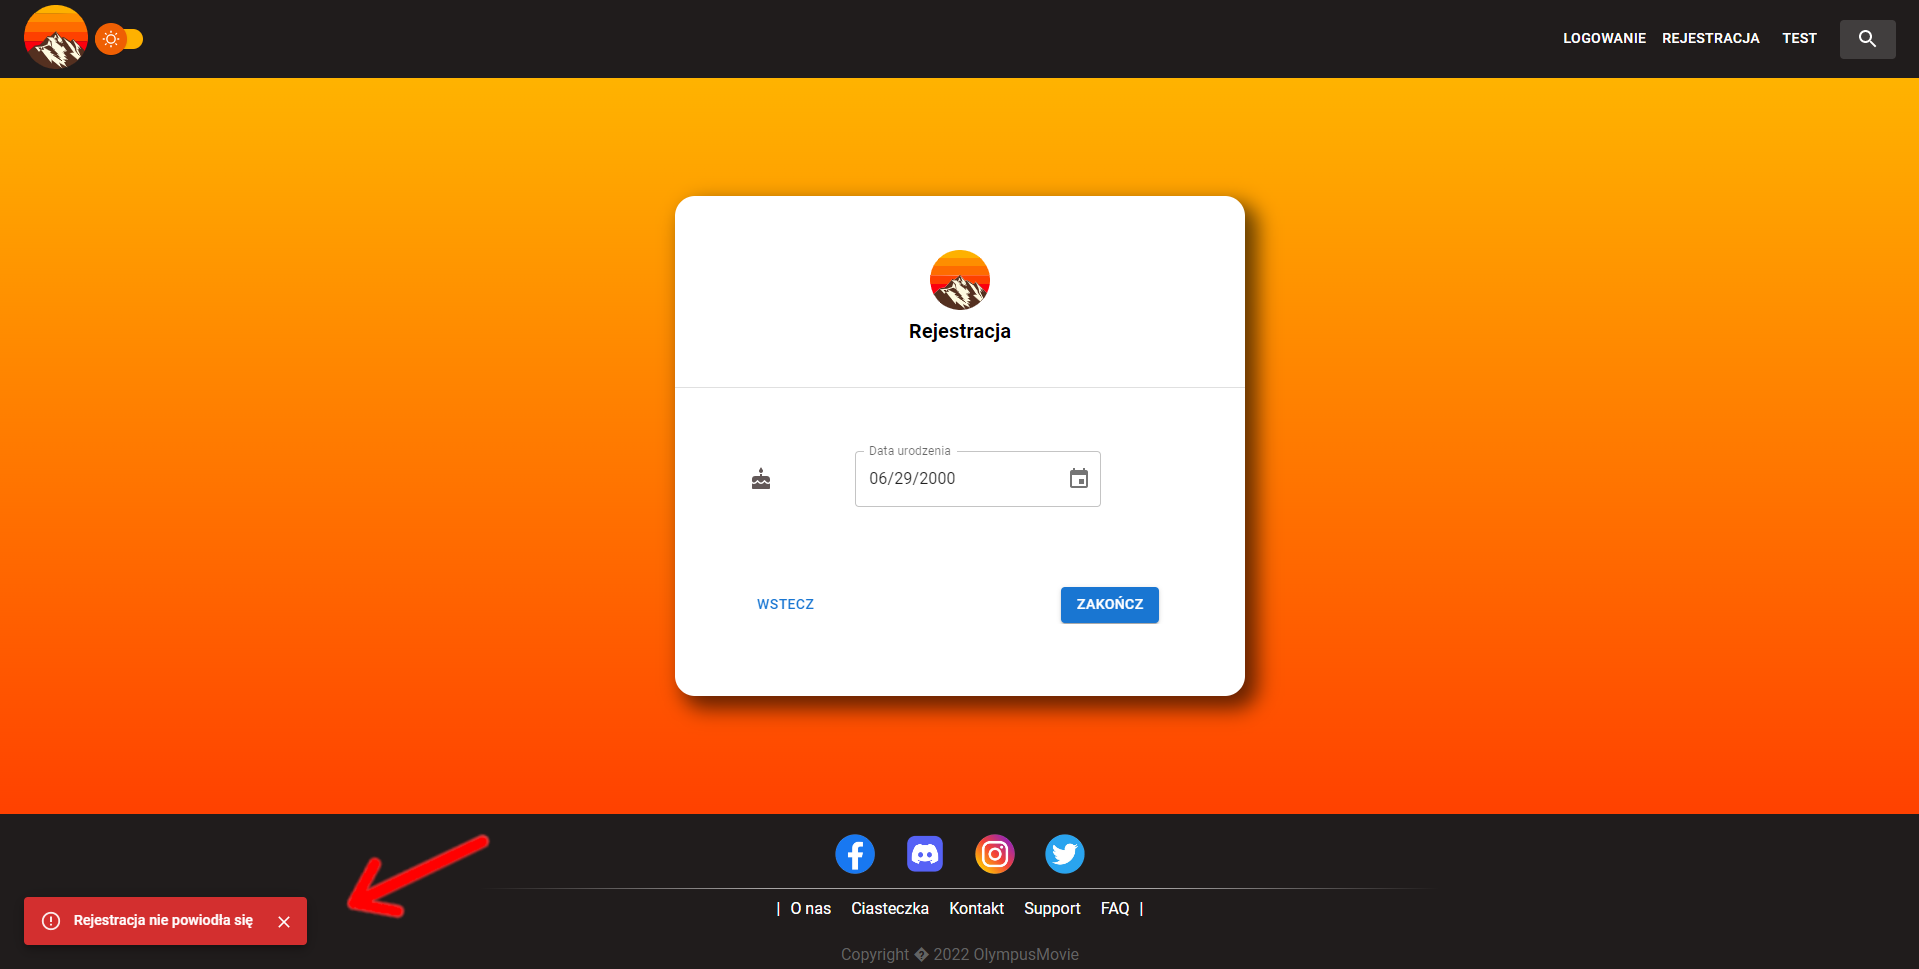
\includegraphics[scale=0.3]{RejestracjaNieudana.png} \linebreak
			

			
			\item Logowanie. \linebreak
			W prawym górnym roku strony kliknąć "LOGOWANIE". \linebreak
			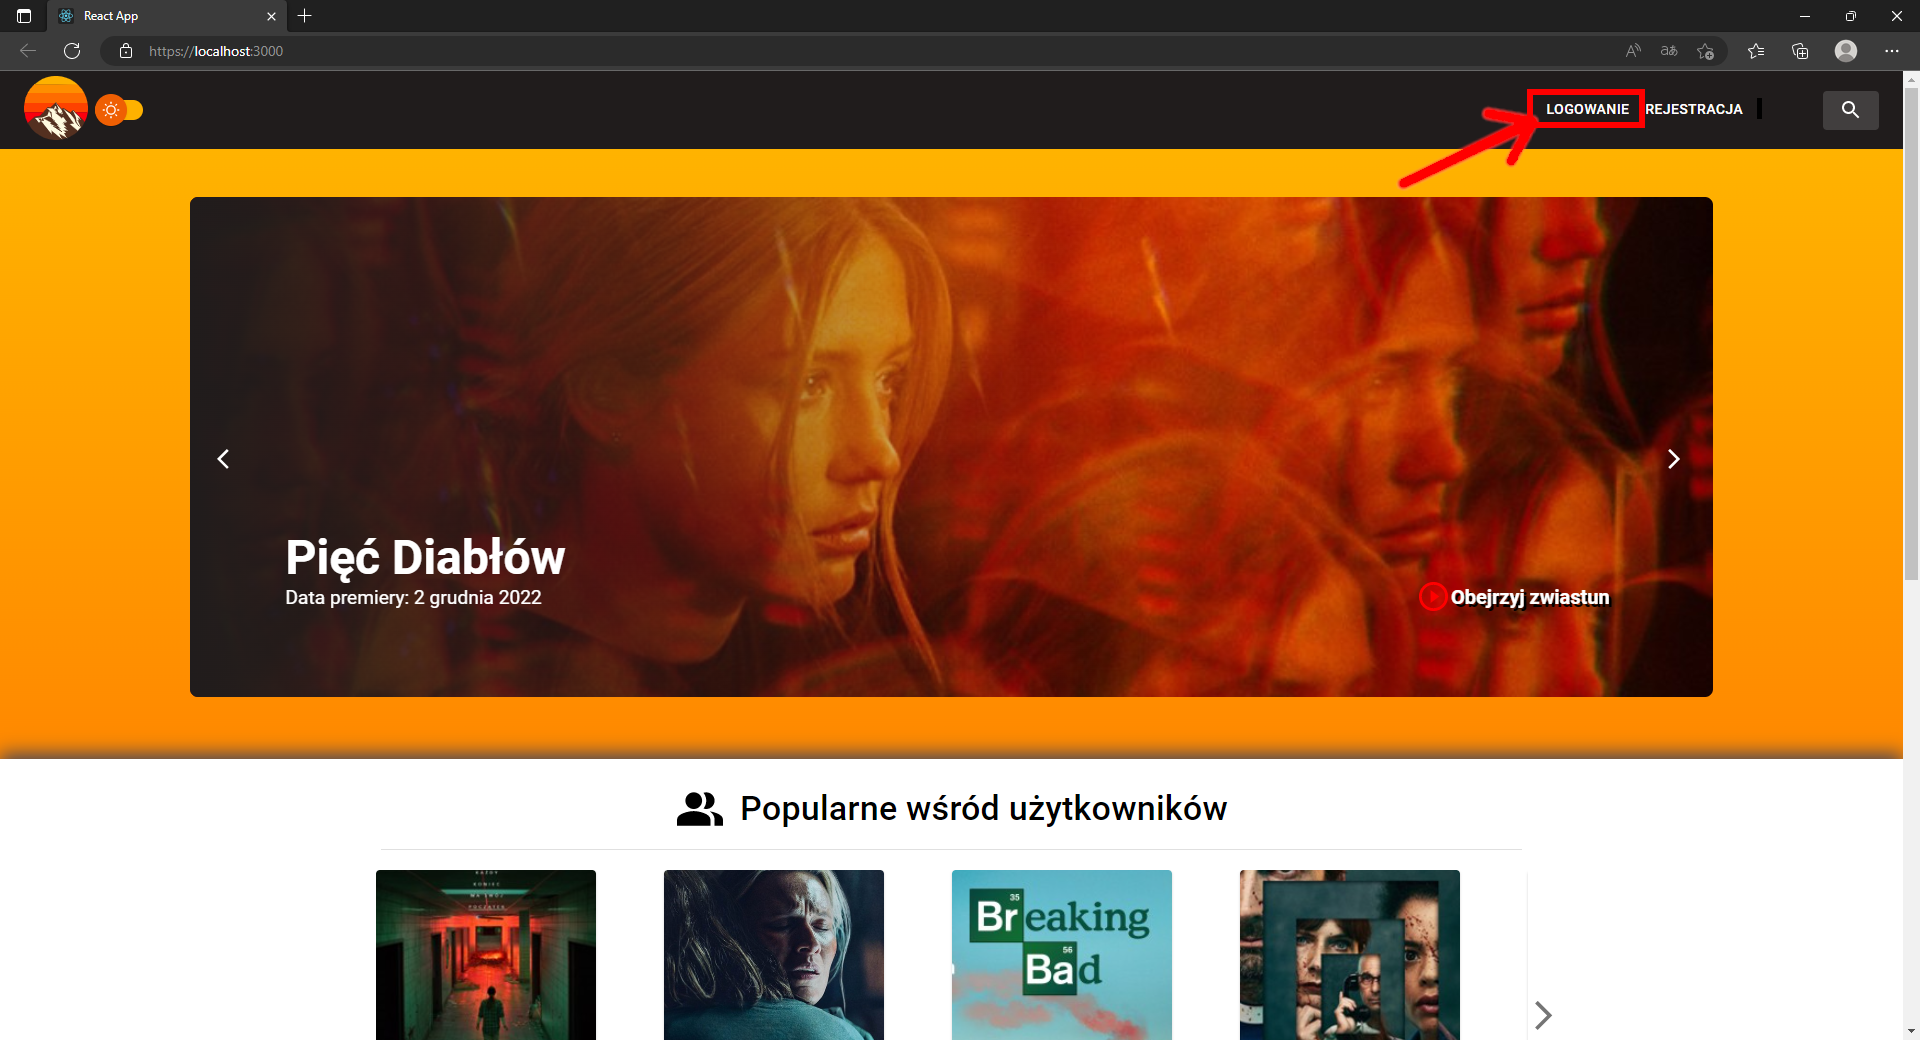
\includegraphics[scale=0.3]{Logowanie1.png} \linebreak
			W wyświetlonym formularzu należy wpisać dane wcześniej utworzonego konta następnie kliknąć "ZALOGUJ SIĘ". \linebreak
			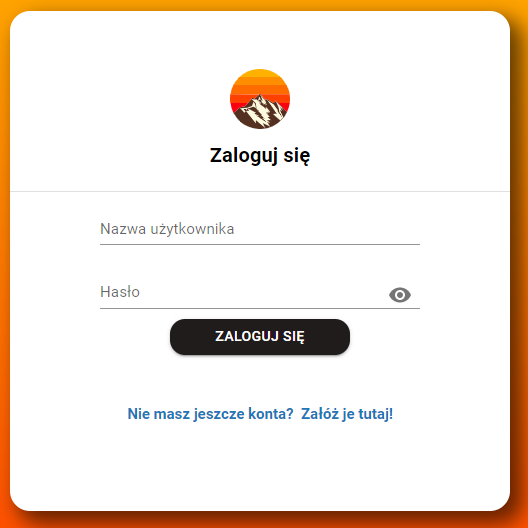
\includegraphics[scale=0.7]{Logowanie2.png} \linebreak
			\item Wyszukanie pozycji na podstawie tytułu.
			W prawym górnym rogu strony należy kliknąć lupę.\linebreak
			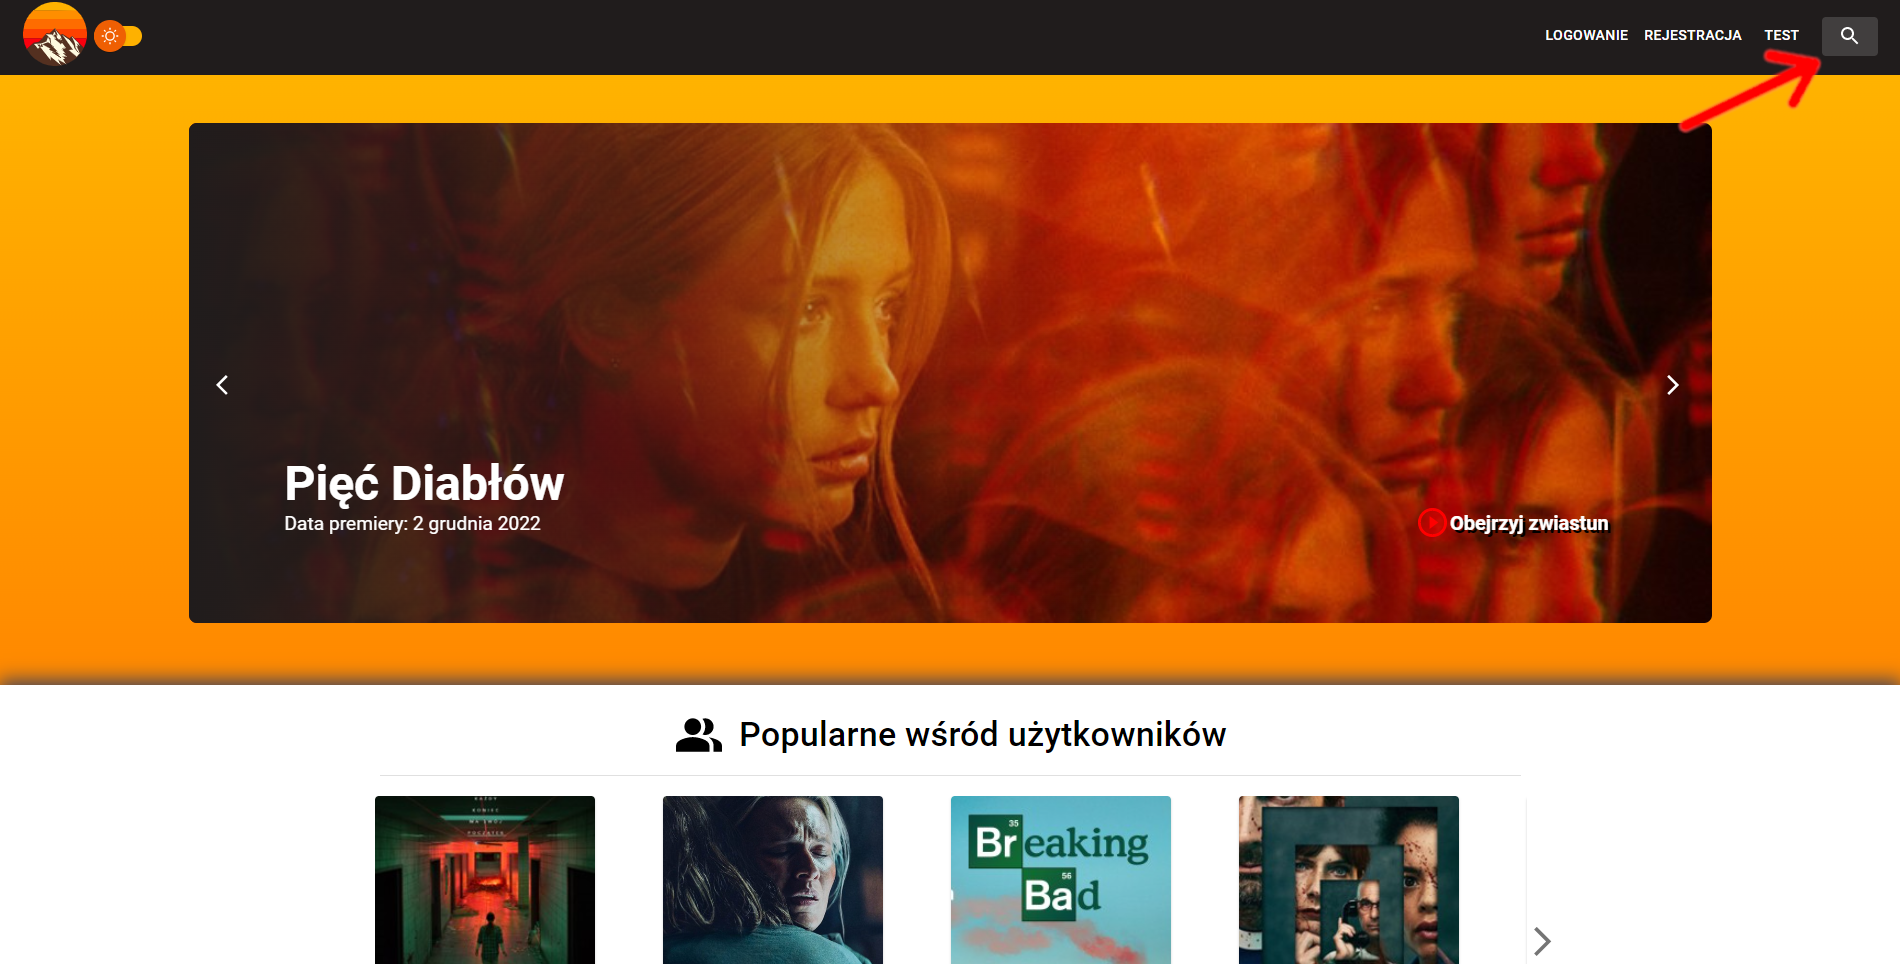
\includegraphics[scale=0.3]{WyszukiwanieTytul1.png} \linebreak
			Następnie w miejscu obok lupy należy wpisać część lub całość tytułu. \linebreak	
			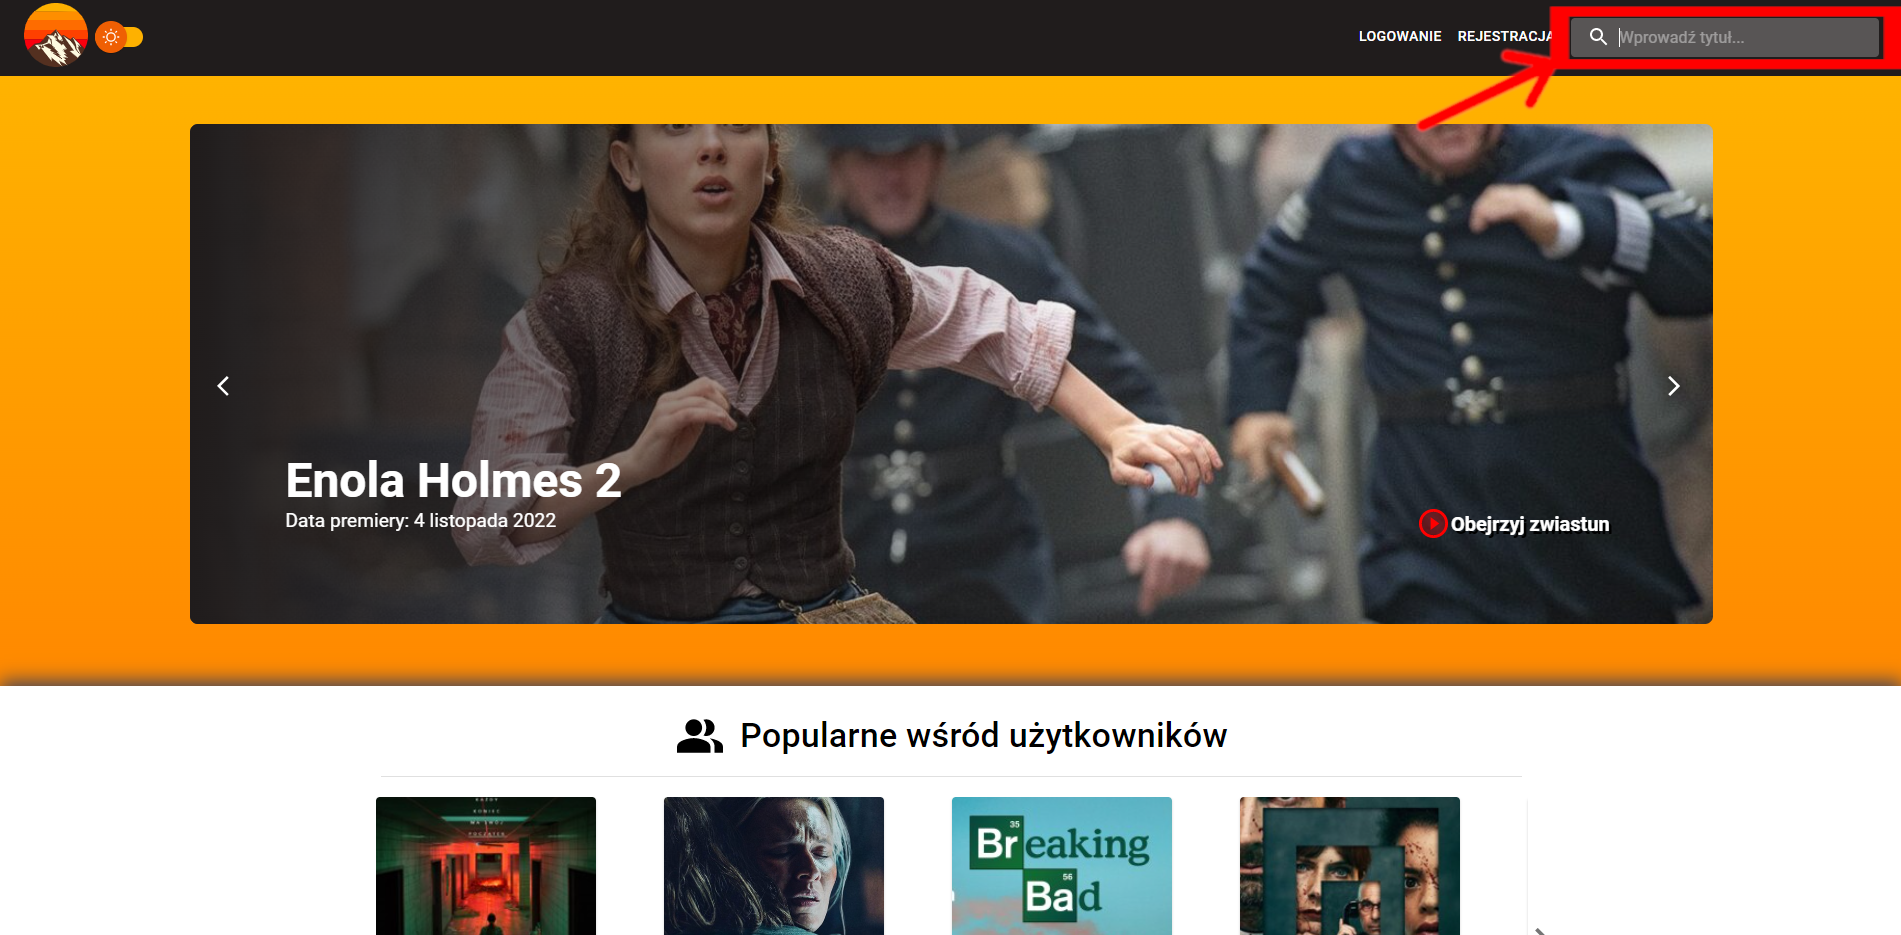
\includegraphics[scale=0.3]{WyszukiwanieTytul2.png} \linebreak
			Po zatwierdzeniu tytuły pasujące do wpisanej frazy tytuły zostaną pokazane zamiast strony głównej. \linebreak
			\item Wyszukanie pozycji na podstawie filtrów.\linebreak
		\end{itemize}
		\subsection{Funkcjonalność użytkownika zalogowanego}
		Użytkownik zalogowany posiada wszystkie funkcjonalności użytkownika anonimowego poza logowaniem, rejestracją i losowaniem nazwy użytkownika podczas rejestracji. Dodatkowo:
		\begin{itemize}
			\item Wylogowanie się.
			\item Otworzenie własnego profilu
			\item Dodanie oceny do pozycji.
			\item Dodanie recenzji do pozycji.
			\item Skomentowanie recenzji.
			\item Dodanie pozycji do jednej z list.
		\end{itemize}		
		\subsection{Funkcjonalność użytkownika administratora}	
		Administrator posiada wszystkie funkcjonalności użytkownika zalogowanego. Funkcje przeznaczone jedynie dla administratora wykonuje się z poziomu API:
		\begin{itemize}
			\item Dodawanie rekordów do baz danych.
			\item Edytowanie rekordów w bazach danych. 
			\item Usuwanie rekordów z baz danych.
		\end{itemize}
	
%	\section{Informacje o wersji}
	
	


	
	
			
		%\subsection{Mapa strony}
		%\subsection{Lista funkcjonalności}
		%\subsection{Wersje językowe}
	%\section{Wymagania techniczne}
		%\subsection{Wsparcie przeglądarek}
	\pagebreak
	\section{Licencje}
		\begin{enumerate}
			\item	Pixabay
			\url{https://pixabay.com/service/terms/#license}, 
			data ostatniej aktualizacji: 13.12.2021
			
			
			\item	Boxicons
			\url{https://boxicons.com/usage#license}, 
			data wejścia na stronę: 18.10.2022
		\end{enumerate}
	
	
	%----------------------------------------------------------------------------------------
	
	%----------------------------------------------------------------------------------------
	%		Bibliography
%	\bibliographystyle{plain}
%	\bibliography{mybib}
	
	%----------------------------------------------------------------------------------------
\end{flushleft}
\end{document}
